\documentclass[11pt, letter]{article}

\usepackage{graphicx}
\usepackage{url}

\title{Decoupled Software Pipelining in LLVM \\
        {\large 15-745 Final Project}}
\author{Fuyao Zhao, Mark Hahnenberg\\
\url{fuyaoz@cs.cmu.edu}, \url{mhahnenb@andrew.cmu.edu}
}
\date{}

\begin{document}

\maketitle

\section{Introduction}
\subsection{Problem}
Decoupled software pipelining \cite{DSWP} presents an easy way to automatically extract thread-level parallelism for general loops in any program.  The compiler does this by examining the dependences of the loops in a given program, 


splitting the instructions of those loops into multiple smaller loops that execute in independent threads, and inserting dependence communication where necessary between these threads so that they remain synchronized.  The full process is described below in detail.  

\subsection{Approach}
We chose to implement DSWP using the general-purpose POSIX threading library (pthreads) and the Low Level Virtual Machine (LLVM) compiler infrastructure.  

\subsection{Related Work}
The initial DSWP has been implemented in the context of the IMPACT research compiler using Itanium platform simulator which has customized hardware-level support. Other works of DSWP including \cite{Sp-DSWP,PS-DSWP} also use hardware simulator.

\subsection{Contribution}
The decision to use LLVM will allow our implementation to be viewed in a context that is more relevant and more widely used than the IMPACT compiler, as LLVM is becoming not only a research but industry standard.  Due to our choice to use pthreads, Our DSWP implementation will also be portable across more platforms than previous implementations since any system that supports both LLVM and POSIX will be able to use our implementation, while former systems were limited to the Itanium platform with customized hardware support.

\section{Design}
\subsection{The Steps of DSWP}
DSWP can be described as a series of steps that first accumulate information about the program, then use that information to the extract the TLP from the program's loops, and finally modifies the program to execute in parallel those portions deemed to be parallelizable.

\subsubsection{Build Program Dependence Graph (PDG)}
In order to correctly insert dependence flows among the independently running sub-loops that are generated we need to enumerate the various dependences among the instructions in each loop within the program.  These dependences can be classified into two categories: data dependences and control dependences.  We build the PDG \cite{PDG} containing this information as our first step as in Figure~\ref{pdg}.

This process is different than how it was described in the paper.  The paper \cite{DSWP-OR} used a method of peeling off the first iteration of the loop and running normal dependence analysis on that graph and then coalescing the duplicated nodes afterward to fit the original graph.  This was difficult in LLVM because of the fact that LLVM is in SSA form, so it would have been unclear as to how to modify the program graph to make this work, a possible solution would be introduce phi node, while our current implementation only support the un-optimized code. 

Therefore, we did this in another way. In addition to the normal PDG, essentially we need the header to have a control dependence on any block that branches either to the exit or to the header.  We do this simply by checking each branch instruction within the loop to see if it goes back to the loop header.  If it does, then we mark the header as depending on that block. 

\begin{figure}
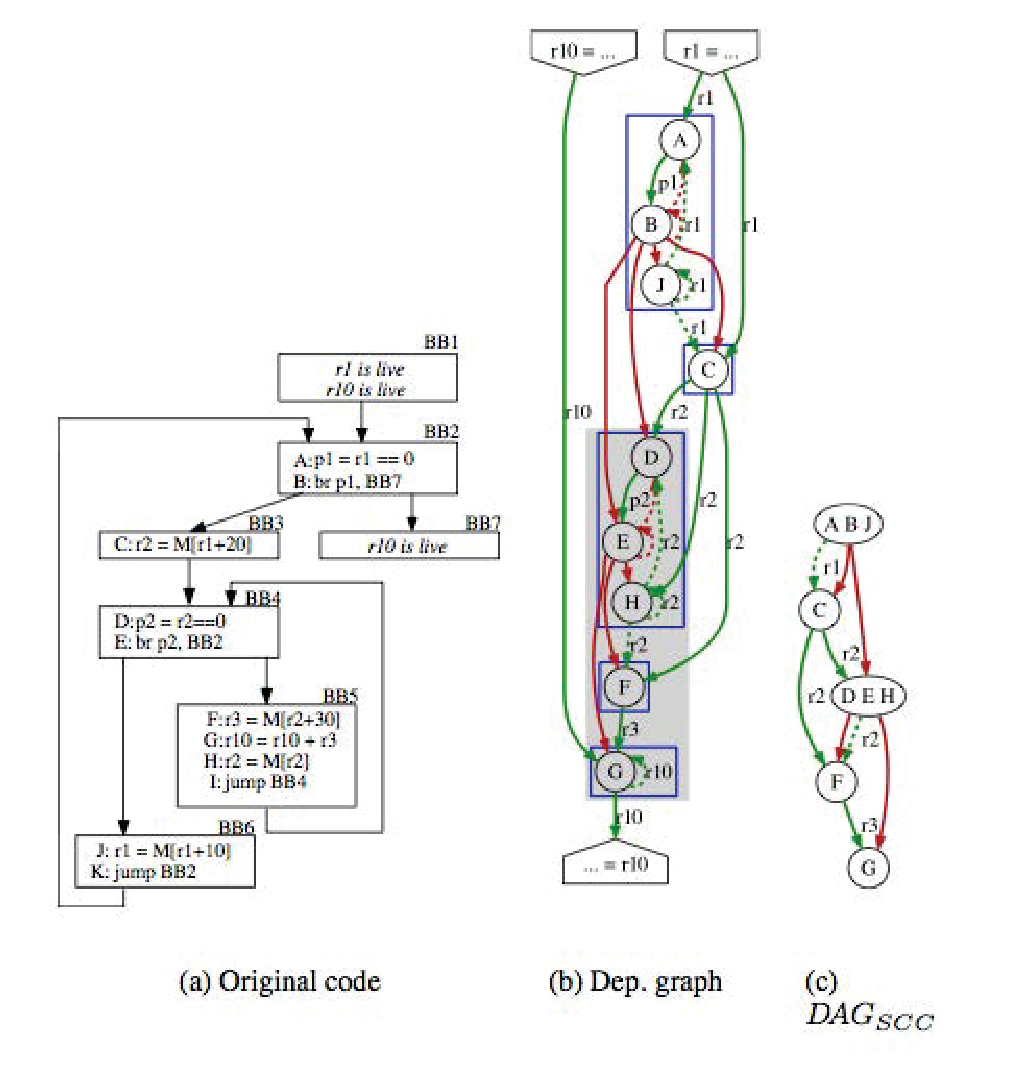
\includegraphics[scale=0.75]{pdg}
\caption{Illustrates the original program (a), the PDG based on that code (b), and the $DAG_{SCC}$ generated using the PDG.}
\label{pdg}
\end{figure}

\subsubsection{Find Strongly Connected Components (SCC) and Coalesce into a DAG}
In the next step, we take the PDG and find the strongly connected components \cite{CLRS} in it.  We do this to ensure that there are no cycles in the resulting graph when we coalesce the nodes, which is necessary to form a pipeline.  Each of these SCCs represents cyclic dependences within the loop, so the compiler requires that these remain in the same thread.  After we have found the SCCs, we coalesce each of them into single nodes to form a DAG.  Refer to Figure~\ref{pdg} for an illustration of this process.

\subsubsection{Assign Partitions of DAG to Threads}
Our goal for the next step is to partition the nodes of the DAG among a fixed set of threads.  A valid partitioning $P$ is such that all of the dependence arcs either are within the same $P_i \in P$ or they go from $P_i$ to $P_j$ such that $i < j$, thus forming a pipeline between the partitions.  We want to choose a partitioning among the threads such that we minimize our overall execution time.  While this general problem is NP-complete \cite{DSWP-OR}, we use the heuristic from the \cite{DSWP-OR} to provide an estimation for a given partition of the DAG. It's basically a gready algorithm which alway try to add the DAG node who has the largest latency.

However, in this model, the communication cost is not considered, which is also a main difference between our implementation and previous one. Many of the partition results we've examined is could improved if the synchronization cost could considered. One possible solution would be to give more priority to the nodes not in current partition, but have more edges to the nodes in current partition in addition to the latency criterion. This idea would be futher experiemnt in the future. 

In addition, we would like to think if there is a better model to formulate our problem in which we could use better algorithm to do thread partitioning. e.g it is possible that split the program into two thread better that split it into three or more thread even we have the thread resouces.

\subsubsection{Split Partitions into Loops}
After we find a valid partitioning of the nodes, we create a new function for each partition and copy in the relevant instructions for those partitions.  In the original thread, we send the addresses of these functions to the waiting threads.

\subsubsection{Insert Dependence Synchronization}
After generating the new functions to be assigned to the separate threads, we need to insert the dependence communication between the partitions. 
% We need some additional control dependences that aren't captured by traditional control dependences. 
 Since different synchronization queues can be used on consecutive iterations, we must synchronized the threads iteration by iteration. See Figure~\ref{sync} for an example of code being split across two threads and the resulting produce and consume sites that must be inserted.

\begin{figure}
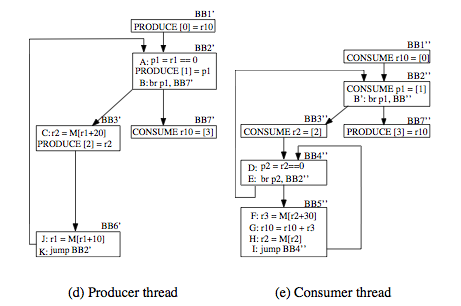
\includegraphics[scale=0.75]{sync}
\caption{Illustrates the splitting of code across threads and the insertion of synchronization primitives (produce (d) and consume (e)).}
\label{sync}
\end{figure}

\subsubsection{Runtime Support}
The compiler needs the support of a runtime library that will manipulate the necessary synchronization primitives.  A separate synchronization library (simple\_sync.c) is linked with the regular source code at compile time.  This library, in turn, uses queue.c as its queue implementation.  We statically create 256 dependence queues.  Each queue has length 32.  If the queue is empty, pop operations will block until a value is pushed into the queue.  If the queue is full, push operations will block until space becomes available.  The locations where produce and consume instructions are inserted into the program during compilation are simply function calls to this library.

At the beginning of each loop the new threads are created and sent the address of the function they are to execute.  Each dependence gets its own queue. We statically create 256 queues to use for the various dependences.  Each produce in the thread that generates the dependence is matched by a single consume in the thread that requires that dependence.

\section{Experimentation}
We built a loadable module for LLVM that can be called as a separate optimization pass.  We then ran this pass on some self-written benchmarks.  We initially intended to run our optimization on the SPEC2006 benchmarks, however, Our current implementation is limited in dependence analysis so that could not used for large program. 

For simple program, our implementation has significant overhead, e.g, for a loop which will caculate the sum from 1 to 10000, the un-optimized code take 0s while our parallezed one take 4s. This is mainly because when the program is splited, one thread basically do loop counter increase and another thread to the sum, and thus we have huge synchronization cost.


\section{Lessons Learned}
Academic papers are not always explicit about the steps they take in their implementations, in order to capture all the neccessary detail, you must be more knowledgeable, e.g to read more papers related to the topic, after that you probably could infer what is really going on there.

Additionally, our software engineering skills could be worked on, specifically our estimation of project size and our time allocation.  This project was a more significant undertaking than we initially thought. (e.g. the code spliting seems to be the simplest part but it take us most time to finish). Currently the project sits at about 2 KLOC and still more could be done.  

\section{Future Work}
We still need to test our implementation more on complex programs, for example, the SPEC2006 benchmarks on multiple platforms, especially machines with higher numbers of cores.  These tests would help us verify that our implementation was correct and it would also gives us a better idea of how a software-only implementation of DSWP compares to unoptimized code as well as hardware-supported DSWP.

Our dependence analysis is limited in several way, we need to have a reasonable solution for the dependencde that DSWP needed, and consider the dependence after we have phi node in the code. In addition, better alias analysis would help us improve the result of dependency, therefore reduce the overhead of synchronization.

Since we have a different implementation of thread synchronization our model for the costs of synchronization could be significantly different from those defined in previous papers. As we mentioned previously, we could investigate these costs further to get more accurate model and better heuristics, thereby improving the quality of our thread partitioning.

The way that we rewrite the program causes a lot of overhead in that we start a group of threads at the beginning of each loop body and then join them at the end of the loop body.  We could reduce this initialization overhead by creating all the threads at the beginning of the program or perhaps lazily when we encounter our first loop body.
% since whether we encounter any loop bodies is undecidable in general. We would then keep those threads throughout the rest of the program, dispatching them to different functions based on whatever loops we encounter. We chose our current implementation because it was much simpler to implement for an initial version.


\section{Conclusions}
Despite the lack of official benchmark results, we can hypothesize that our software-only implementation of DSWP will not be able to compete with a similar implementation with custom hardware support.  However, we have presented a method to extract thread-level parallelism from general loop bodies in a more platform-independent fashion than the previous state-of-the-art.

Therefore, we think that if DSWP is going to be widely used by industrial, it must solve the problem of communication overhead, as we discussed in the report, we need either improve the thread partitioning significantly or add hardware support,  though it has shown its promise in several academic papers. 

\bibliographystyle{plain}
\bibliography{bib}

\subsection*{Distribution of Total Credit}
Fuyao implement framework of DSWP and componenent for dependence analysis, SCC/DAG, thread partitioning, loop spliting and synchronization. Mark impelmented the runtime support for multithreding based on pthread, he also contributed to the sychronization part, and managed write-ups.

\end{document}
